% !TEX encoding = UTF-8 Unicode
% !TEX root = ../Rapport/rapport.tex


Nous avons décidé d'implémenter tous les algorithmes suivants en langage C pour des raisons d'efficacité.

\section{Programmation dynamique}
La programmation dynamique est un paradigme d'algorithmes exacts qui consiste à plonger le problème dans sa généralisation. Le principe est d'utiliser une fonction de récursion pour calculer la solution optimale d'un sous-problème du problème courant. À partir de la solution de ce sous-problème, on obtient la solution d'un sous-problème plus grand, etc, jusqu'à résoudre le problème de départ.

%Espace de recherche, sous-ensemble de l'espace de recherche

\subsection{Problème de la partition}

\subsubsection{Description du problème}
Le problème de la 2-partition de $n$ objets consiste à trouver deux sous-ensembles de ces $n$ objets tel que chacun des sous-ensembles ait le même poids. Les poids de chacun des objets étant des valeurs entières, pour qu’il existe deux sous-ensembles distincts ayant le même poids, il faut que la somme des poids des objets soit paire.

\subsubsection{Algorithme de programmation dynamique}
Prenons l'algorithme de résolution présenté dans la section théorique (cf \ref{algo_dyn_partition}) et rappelé ci-dessous. Cet algorithme est un algorithme exact admettant une complexité en $O(n.P)$ avec $n$ le nombre d'objets et $P$ la somme des poids de tous les objets.
\begin{algorithm}[H]
	\caption{Partition}
	\label{algo_dyn_partition}
	\begin{algorithmic}[1]
		\STATE $P \leftarrow \sum_{i \in \mathbb{[}1, n \mathbb{]}} p(a_i)$
		\IF{$P \equiv 1 \pmod{2}$}
			\RETURN Pas de solution
		\ELSE
			\FOR {$j \in \mathbb{[}0,P/2\mathbb{]}$}
				\IF{$j = 0$}
					\STATE $T(0, j) \leftarrow \TRUE$
				\ELSE
					\STATE $T(0, j) \leftarrow \FALSE$
				\ENDIF
			\ENDFOR
			\FOR{$i \in \mathbb{[}1, n \mathbb{]}$}
				\FOR{$j \in \mathbb{[}0, P/2\mathbb{]}$}
					\STATE $T(i, j) \leftarrow [\left (j = 0) \vee (j = p(a_i)) \vee (T(i-1, j)) \vee (T(i-1, j-p(a_i))) \right]$
				\ENDFOR
			\ENDFOR
			\IF{$T(n, P / 2) = \FALSE$}
				\RETURN Pas de solution
			\ELSE
				\RETURN Partition-Solution($n$,$\frac{P}{2}$,$T$)
			\ENDIF
		\ENDIF
	\end{algorithmic}
\end{algorithm}

\begin{algorithm}
	\caption{Partition-Solution}
	\label{recsol}
	\begin{algorithmic}[1]
	\REQUIRE
		\IF{$i = 0$ \OR $j=0$}
			\RETURN $S$
		\ELSE
			\IF{$T(i-1,j) = \FALSE$}
				\RETURN $a_i \cup$ Partition-Solution($i-1$,$j-a_i$,$T$)
			\ELSE
				\RETURN Partition-Solution($i-1$, $j$, $T$)
			\ENDIF
		\ENDIF
	\end{algorithmic}
\end{algorithm}




\subsubsection{Implémentation}
Cet algorithme a été implémenté de manière naïve : comme présenté en partie théorique et ci-dessus.
Nous avons donc codé la matrice intégralement.

\subsubsection{Tests}
La phase de tests dont la courbe ci-dessous résulte a été limitée par la capacité de la mémoire vive de notre ordinateur de test.
\begin{figure}[H]
	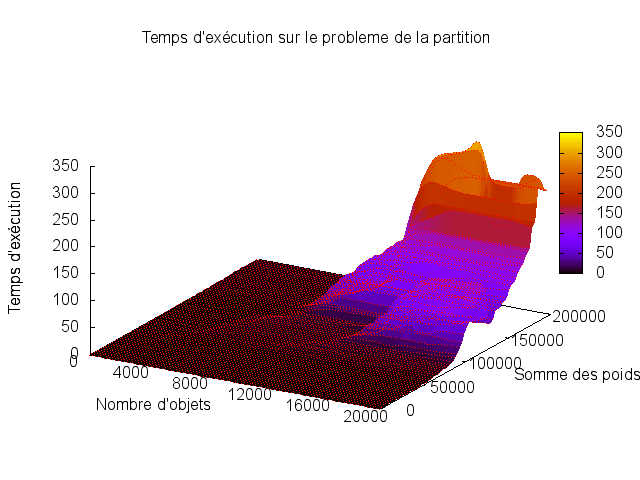
\includegraphics[width=\linewidth]{../pratique/prog_dynamique_dev/res/partition.png}
\end{figure}


\subsection{Problème du sac à dos}

\subsubsection{Description du problème}
Le problème du sac à dos consiste à vouloir mettre des objets ayant chacun différents volumes et utilités dans un sac à dos à volume limité. Le but est d'obtenir un sac à dos rempli avec une utilité maximum.

\subsubsection{Algorithme de programmation dynamique}
Prenons l'algorithme de résolution présenté ci-dessous servant à résoudre le problème du sac à dos dans lequel nous pouvons mettre plusieurs fois le même objet. Cet algorithme est un algorithme exact admettant une complexité en $O(n.V^2)$ avec $n$ le nombre d'objets et $V$ le volume du sac à dos. Notons que la borne (pire des cas) est atteinte si tous les objets sont de volume 1.
\begin{algorithm}[H]
	\caption{Sac à Dos}
	\label{algo_dyn_bag}
	\begin{algorithmic}[1]
		\FOR {$j \in \mathbb{\{}1, \ldots, volumeMax \mathbb{\}}$}
				\STATE $T[0, j] \leftarrow 0$
		\ENDFOR
		\FOR{$i \in \mathbb{\{}1, \ldots, n \mathbb{\}}$}
			\FOR{$j \in \mathbb{\{}1, \ldots, volumeMax \mathbb{\}}$}
				\IF{$j \neq 1$}
					\STATE $T[i, j] \leftarrow T[i, j-1]$
				\ENDIF
				\FOR{$k \in \mathbb{\{}0, \ldots, volumeMax/volume[i] \mathbb{\}}$}
					\STATE $T[i,j] \leftarrow \max(T[i,j], T[i-1,j-k \times volume[i]] + k \times utilite[i])$
				\ENDFOR
			\ENDFOR
		\ENDFOR
	
	\RETURN $T[n,volumeMax]$
	\end{algorithmic}
\end{algorithm}



\subsubsection{Implémentation}\label{bag_impl}
Etant donné que pour calculer une nouvelle ligne, il nous suffit de regarder dans la précédente, nous 
avons décidé de ne pas stocker la matrice intégralement mais uniquement les deux dernières lignes.
Ainsi, pour obtenir la solution, nous devons stocker les solutions temporaires dans chaque case.
Pour cela, nous avons utilisé une liste simplement chaînée.

\subsubsection{Tests}
Sur la courbe suivante, nous remarquons que le volume du sac influe plus que le nombre d'objets sur le temps d'exécution. Ce qui confirme nos attentes théoriques.
\begin{figure}[H]
	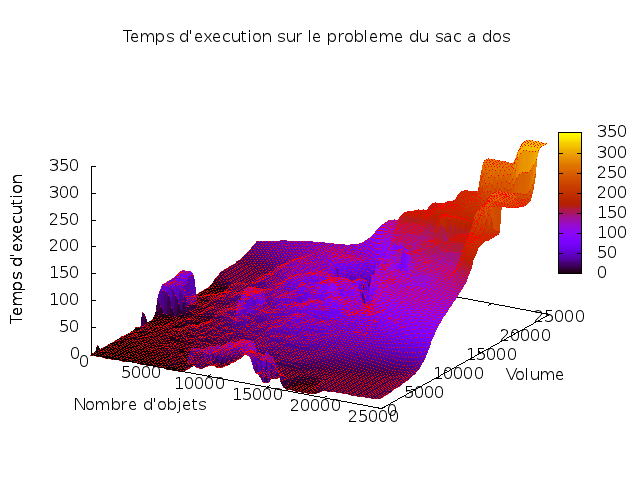
\includegraphics[width=\linewidth]{../pratique/prog_dynamique_dev/res/bag.png}
\end{figure}


\subsection{Problème du voyageur de commerce}

\subsubsection{Description du problème}
Le problème du voyageur de commerce consiste à trouver un cycle hamiltonien de poids minimum.
\subsubsection{Algorithme de programmation dynamique}

\begin{algorithm}[H]
	\caption{Voyageur de Commerce}
	\begin{algorithmic}[1]
		\FOR{$i \in \{1,...,n\}$}
			\STATE $C(\{0\},i) \leftarrow \omega(0,i)$
		\ENDFOR
		\FOR{$i \in \{2,...,n\}$}
			\FOR{$S \subseteq \{1,...,n\} : |S| = i$}
				\FOR{$j \in V \setminus S$}
					\STATE $C(S,j) \leftarrow \min\limits_{k \in S \setminus \{0\}}(C(S\setminus\{k\},k) + \omega(k,j))$
				\ENDFOR
			\ENDFOR
		\ENDFOR
		\RETURN $\min\limits_{i\in V\setminus\{0\}}(C(V\setminus\{i\},i) + \omega(i,0))
	\end{algorithmic}
\end{algorithm}




\subsubsection{Implémentation}
Comme pour le problème du sac à dos, nous n'avons pas conservé l'ensemble de la matrice.
Ici, nous ne gardons que les colonnes dont l'ensemble $S$ a pour arité la taille des chemins en cours
de calcul moins un.
De plus, étant donné que le nombre de colonnes à générer pour une nouvelle cardinalité est difficile à prévoir,
nous avons utilisé des listes chaînées de manière à stocker celles-ci sans pour autant allouer plus de mémoire que nécessaire.


\subsubsection{Tests}
Comme visible sur la courbe, il est très difficile de résoudre ce problème via la programmation dynamique. En effet dès que le nombre de sommets dépasse 15, le temps d'exécution n'est plus raisonnable.

\begin{figure}[H]
	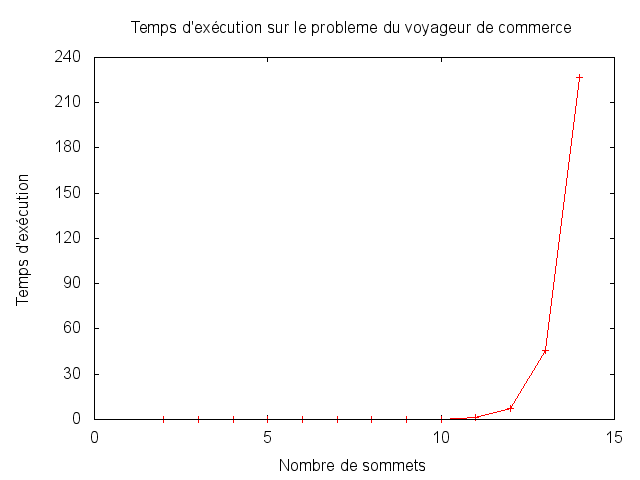
\includegraphics[width=\linewidth]{../pratique/prog_dynamique_dev/res/tsp.png}
\end{figure}


